\chapter{Application}
\section{Data Explanation}
\label{sec:data}
\begin{comment}
We have now laid down the theory of what we want to do describing all of the choices we may need to make, so now we will put it in action. The data that we will apply it to is a dataset from M.D Anderson Cancer Center. The data is a collection of about 1500 patients at MD Anderson who have breast cancer that has metastasized to the brain, about 100 clinically relevant covariates, along with their survival status and time.
\end{comment}
Now that the theory is in place, we can apply it to some real data. The dataset that I chose to analyze is a dataset from MD Anderson Cancer Center, with permission from Dr. Bugano, Dr. Ibrahim, and Dr. Hess. The IRB protocol is RCR03-0931. This dataset has historical records of 1514 MD Anderson patients who have had breast cancer that has metastasized to the brain from October 2009 to December 2012. Metastases are often shortened in speech and in paper to the word ``mets''. The dataset consists of 111 covariates, with missingness ranging from 0 to 99\%. Some predictors are metadata, and rare tests, so they will not be considered. Ignoring these, so the missingness in the useful data ranges from 0 to 65\%. Included in these are 90 different covariates, a few different treatments, as well as survival endpoints (which are all observed). The data can be broken down into a few broad categories, as can be seen in table \ref{table:cats}.There are too many covariates to completely explain here, but I�ve listed the ones relevant to our models in table \ref{table:importantvars}

\begin{table}[ !ht]
\centering
\begin{tabular}{|c|c|}
\hline
Type                                                                            & Example                                                                       \\ \hline
Subject data                                                                    & Age range, race, date of birth                                                \\ \hline
Breast Cancer data                                                                     & TNM staging, type, receptor status                                            \\ \hline
\begin{tabular}[c]{@{}c@{}}Pre brain mets\\ data\end{tabular}                   & Treatment types                                                               \\ \hline
\begin{tabular}[c]{@{}c@{}}Post brain mets\\ clinical observations\end{tabular} & Seizures, headache, nasuea                                                    \\ \hline
\begin{tabular}[c]{@{}c@{}}Post brain mets\\ data\end{tabular}                  & \begin{tabular}[c]{@{}c@{}}Treatment type, \\ type of brain mets\end{tabular} \\ \hline
Survival data                                                                   & Survival time after brain mets, censoring indicator                           \\ \hline
\end{tabular}
\caption{Data Categories and Examples}
\label{table:cats}
\end{table}

  \begin{table}[!ht]
\centering
%\adjustbox{max height=\dimexpr\textheight-5.5cm\relax,
 %          max width=\textwidth}{
\begin{tabular}{|c|c|c|}
\hline
Name        & \begin{tabular}[c]{@{}c@{}}Percent \\ Missing\end{tabular} & Meaning                                                                                                                                             \\ \hline
capeothno   & 18\%                                                        & \begin{tabular}[c]{@{}c@{}}Indicator: Capecitabine, other, or no chemotherapeutic\\ treatment. Treatment variable 1\end{tabular}                     \\ \hline
lapatrasno  & 18\%                                                        & \begin{tabular}[c]{@{}c@{}}Indicator: Lapatinib, Trastuzumab, or no HER2 treatment.\\ Treatment variable 2\end{tabular}                             \\ \hline
controlled  & 12\%                                                        & Indicator: Extracranial progression of brain mets                                                                                                   \\ \hline
%her2        & 10\%                                                        & Indicator: HER2 receptor status                                                                                                                     \\ \hline
hrher2      & 5\%   													& \begin{tabular}[c]{@{}c@{}}Categorical variable: The hormonal receptor and \\ HER2 receptor status of the subject\end{tabular}  						\\ \hline
braintype   & 4\%                                                        & Categorical: Single, multiple, Leptomeningeal disease                                                                                               \\ \hline                                                                       
timedx      & 1\%                                                        & \begin{tabular}[c]{@{}c@{}}Indicator: Time (years) from breast cancer diagnosis to brain\\ mets diagnosis greater or less than 6 years\end{tabular} \\ \hline
site5       & 1\%                                                     & Indicator: First metastasis was to brain                                                                                                            \\ \hline
race2       & 0\%                                                          & Categorical: White, Black, Hispanic, other                                                                                                          \\ \hline
priorn      & 0\%                                                          & \begin{tabular}[c]{@{}c@{}}Indicator: Number of prior treatments in metastatic setting \\ before brain mets\end{tabular}                            \\ \hline
os          & 0\%                                                          & Overall survival (months)                                                                                                                           \\ \hline
dead        & 0\%                                                          & Indicator: death indicator                                                                                                                          \\ \hline
agebrainmet & 0\%                                                        & Indicator: Age greater or less than 60 at time of brain mets                                                                                        \\ \hline

\end{tabular}
%}
\caption{Table of important covariates to be used in the analysis}
\label{table:importantvars}
\end{table}

To get a feel for how the data is missing, in figure \ref{fig:missingplot} we see a plot of the missingness in the data. There are certainly large swaths and groups of covariates that were not collected, but overall, there seems to be no real pattern in the way the data is missing.
\begin{figure}[h!]
  \centering
    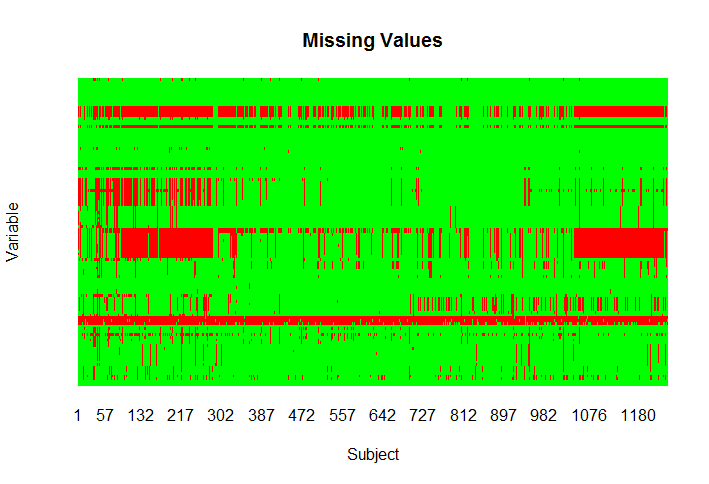
\includegraphics[width=0.8\textwidth]{missingvalues_plot.png}
  \caption{Visualization of missingness in the cancer dataset}
\label{fig:missingplot}
\medskip
\small
Along the horizontal axis is the subject, and the vertical axis are the covariates. Black denotes observed values whereas white is missing. The covariates with the highest missingness are three genetic measures, as well as some clinical assessments.
\end{figure}

This data is exemplary for demonstrating thesis ideas because it is a large retrospective study (pulled from a database), survival amenable, has missingness that is a prime candidate for imputation, and has treatment variables that are not given in an RCT.

Our first step is to clearly define what we would like to find. We will answer two separate questions in the section. In the first, we will explore the treatment effect of Capecitabine (a chemotherapeutic agent) versus other chemotherapeutic agents versus no treatment. In the second, we will look at the effect of two HER2 directed drugs (Lapatinib versus Trastuzumab) versus no HER2 targeted drugs in a subset of the patients who are HER2+.

It isn't vital to understand the entirety of cancer and its treatments for understanding this analysis, but the interested reader may want to look at appendix \ref{app:apdxb} for a very basic overview of breast cancer and the methods of how different drugs work. For a much more detailed analysis and other clinically relevant questions, see the upcoming paper by Bugano, Hess, and Berliner. This is the project that this research was forked off of.

\section{Imputation}

We first need to impute the missing data. This is a challenging task, because of the attention and care that needs to be given to imputing about 90 covariates with missing data. Although we will not be using all 90 covariates, it is important that we impute them, and do so properly. We need them because; they have the potential to be useful as predictors for other covariates, they might be something we are actually analyzing (now or later), we have spent the money to collect the data, and it strengthens the MAR assumption. As well, it is my opinion (and probably a consensus among applied statisticians) that is better to have too many covariates than not enough. After all, variable selection can be performed if there are too many covariates. 

Our data is quite high dimensional, and there are a many binary variables as well as a handful of strictly positive covariates, thus JM imputation seems inappropriate. Instead, FCS models seem better suited. We will be using the R package mice \cite{VanBuuren2011} because it is easy to use yet powerful.  There are other software implementations in different languages (such as PROC MI in SAS, ICE in Stata, and package mi in R), but I found mice to be the most flexible while also being powerful and easy to use.


The first task we need to do is to assess the missing data mechanism. As we have discussed before, there is no formal statistical test to determine what the mechanism is. It is very unlikely that the data is MCAR (which we typically associate with random/accidental deletion), so it is between MAR and MNAR. We have so many different covariates, and it could reasonably be assumed that the missing data we have could be explained by the type of disease, its stage, the subject's age, their standardized assessment, and their survival time, among other things which we have collected. So it would be reasonable to assume that the missing data mechanism is MAR, and thus imputation can be confidently used.
%spineplots here?

Now that the missing data mechanism has been assessed, the imputations need to be set up. For each covariate with missingness, we need to decide the form of the imputation model that will be used for imputation, and what predictors will be used in it. Most of the covariates that needed imputation were either binary or categorical, so the most popular model chosen were logistic regression, multinomial logit regression, or predictive mean matching. The method that was most appropriate for each situation was chosen. The continuous variables were often selected via regression or predictive mean matching. I decided to be very forgiving, and use nearly every reasonable predictor for each missing covariate. I did this to bolster the MAR claim, and avoid variable selection. Van Buuren proposes measures called influx and outflux to determine how worthy and connected each covariate will be as a predictor \cite{VanBuuren2012}. This information was used to remove 11 covariates that were very poor for prediction.
\begin{comment}
\begin{table}[ !ht]
\centering
\begin{tabular}{rrrr}
  \hline
 & Percent Observed & influx & outflux \\ 
  \hline
ki67 & 0.17 & 0.83 & 0.12 \\ 
  brca & 0.05 & 0.95 & 0.04 \\ 
  p53 & 0.01 & 0.99 & 0.01 \\ 
  symptoms & 0.59 & 0.37 & 0.35 \\ 
  seizures & 0.58 & 0.38 & 0.34 \\ 
  headaches & 0.58 & 0.38 & 0.34 \\ 
  nausea & 0.58 & 0.38 & 0.34 \\ 
  chocking & 0.58 & 0.38 & 0.34 \\ 
  balance & 0.58 & 0.38 & 0.34 \\ 
  weakness & 0.58 & 0.38 & 0.34 \\ 
  language & 0.58 & 0.38 & 0.34 \\ 
  cognition & 0.57 & 0.38 & 0.34 \\ 
  ECOG & 0.35 & 0.62 & 0.16 \\ 
  gpaecog & 0.35 & 0.62 & 0.16 \\ 
  gpasum & 0.31 & 0.65 & 0.11 \\ 
   \hline
\end{tabular}
\caption{Percent observed and influx and outflux of the worst predictors. Ki67, brca, and p53 are cancer markers, ECOG and GPA are performance scores}
\label{table:flux}
\end{table}
\end{comment}
Once the model and predictor choices were made, the imputations were run and tuned, and checked by trial and error. This took a considerable amount of time, because after every change made, the algorithm needed to be reran and the convergence and imputations needed to be assessed. As well, changes in model specification were rarely localized to that variable, and often affected others. 

It took about three weeks to set up and check the models. This was because the number of covariates was large, and checking the imputations after a change was time consuming. It would not take this long for a smaller dataset. Creating valid imputations is a skill that lies somewhere between an art and a science, so it takes the theory to know what to do, and trial and error to see if you've done it correctly.


For the final MI dataset, it was decided to impute $m=50$ datasets and 40 iterations for each. Research by White et. al  says that you should choose $m$ to be about 100 times the percentage of incomplete cases (for the analysis at hand) \cite{White2011a}. The data used in our analyses had about 30\% missingness, so imputing 50 datasets was the chosen number. Mice generally converges quickly (within 5 or 10 iterations), but by setting the number of iterations so high (40), it is as if we are setting a burn in period, and then taking our sample.  

After the final imputation model for each covariate with missingness has been set up, we need to run it and save the results. For 50 datasets, 40 iterations, the algorithm runs in about 4 hours, and for 50 datasets with 100 iterations, it took 11.5 hours on a computer with 4 GB of ram and 4 cores. While this seems like a long time, this process only needs to be done once and requires no human interaction, so it can be run overnight and then never need to be touched again. The imputations were run for 100 iterations to see how the run time scaled, as well as to check how the chains behaved and to see how the analyses differed. The results between 50 and 100 iterations were very similar. As well, there is hardly any confidence to be gained going from 50 to 100, and having such large objects in memory can be harder to work with. This is why 50 MI datasets, iterated 40 times each were chosen.

We need to check our final imputations for convergence, reliability, and validity. Convergence is assessed by looking at the trace plots of the imputed value by iteration. According to van Buuren ``the different streams should be freely intermingled with each other, without showing any definite trends. Convergence is diagnosed when the variance between different sequences is no larger than the variance with each individual sequence'' \cite{VanBuuren2011}. This may be hard to visualize all at one time because for each variable, there will be 50 time the number of missing data values for that covariate, so many authors suggest checking the plots of the chain mean and standard deviation by iteration instead. For continues variables, the chains are checked to see how the variance between and within changes at each iteration, as well as to ensure the chains show no pattern.

Diagnosing convergence for binary and categorical variables is a bit tricky, because the mean of a categorical variable is nonsensical, but we can get a good idea of convergence by looking at if the variance remains constant. And for binary variables, knowing how the groups are coded and looking at where the means are can give us an idea of healthy convergence. For example, in the cancer dataset, the variable HER2 is coded as 1 for being HER2 negative and 2 for positive. In the available cases, the split between being HER2 negative and positive is about 60 to 40. Thus, is we were to look at the average of the chains groups, we would expect it to be around 1.4. Seeing something radically different than this (perhaps a mean of 1.9) might suggest the imputation was done wrong, because the group percentages are not near what they should be. We can assess the convergence of the binary variable also by checking how its variance changes by iteration. Large changes from groups by iteration will be noted as large changes in the variance plots, whereas staying constant indicates that the draws are remaining relatively stable.

There are 80 plots to check, they cannot all be shown in this paper, but all of them have been checked. Some interesting ones may be seen in figure \ref{fig:traceplot1} and \ref{fig:traceplot2}. Looking at these plots, convergence certainly seems to be the case.  Other authors suggest using a more formal statistical tests such as $\hat{R}$, but since most of our interesting variables are categorical, this does not make much sense. 

%change these plots
\begin{figure}[h!]
  \centering
    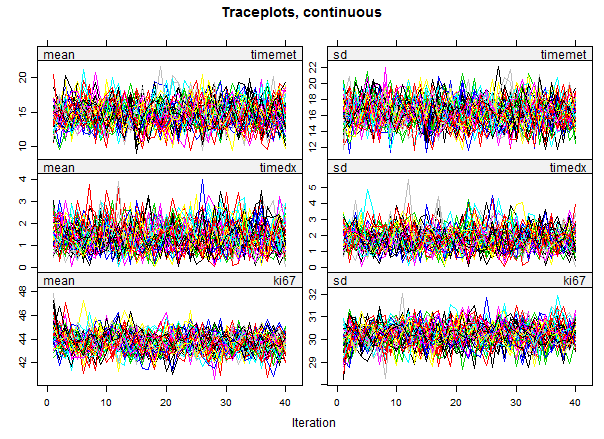
\includegraphics[width=0.8\textwidth]{traceplots1.png}
  \caption{Selected plots of continuous variable imputation mean and standard deviation by iteration}
\label{fig:traceplot1}
\end{figure}


\begin{figure}[h!]
  \centering
    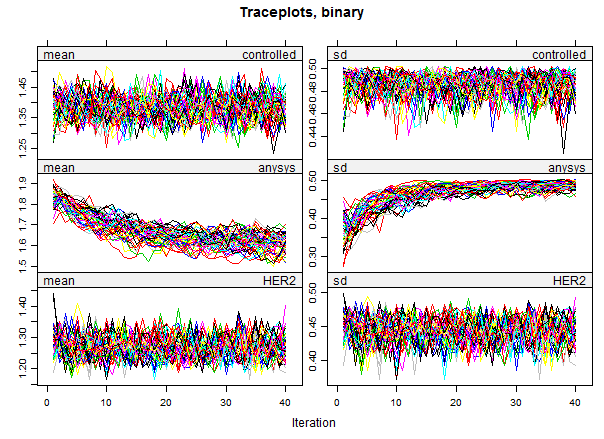
\includegraphics[width=0.8\textwidth]{traceplots2.png}
  \caption{Selected plots of binary variable imputation mean and standard deviation by iteration}
\label{fig:traceplot2}
\end{figure}


Once the convergence is diagnosed, the validity of the imputations needs to be inspected.  Diagnostic plots are viewed to ensure that the imputed data is similar enough to the real data. Common plots include density plots of each MI dataset compared to the complete cases, as well as bivariate scatterplots for imputed variables. < A few of the plots have been replicated here!!! Still need to do this>. Once again, all of the plots cannot be displayed in this paper, but some important ones are recreated. As we can see, not all of the imputed data follows the distribution of the observed data exactly, but for the majority of the plots, the data look like they could have been real data had they not been missing. Now that we have verified the data for convergence and validity, we may run the analyses on the $m=50$ datasets, which we will do in the coming sections.
%%%%%%%%%%
%%%NEED TO DO THE PLOTS
%%%%%%%%%%
Before we move on to the analyses though, let�s have a look at the breakdown of the data. In table \ref{table:chartab} we can see how the MI data compares to the available case data, broken down by if the subject had any systemic therapy. This was computed via the stacked method.
\begin{table}[!ht]
\centering

\begin{tabular}{|r|l|l|l|l|}
\hline
\multicolumn{1}{|l|}{}                            & \multicolumn{1}{c|}{\begin{tabular}[c]{@{}c@{}}Sys therapy \\ available case\end{tabular}} & \multicolumn{1}{c|}{\begin{tabular}[c]{@{}c@{}}Sys therapy \\ MI\end{tabular}} & \multicolumn{1}{c|}{\begin{tabular}[c]{@{}c@{}}No Sys therapy \\ available case\end{tabular}} & \multicolumn{1}{c|}{\begin{tabular}[c]{@{}c@{}}No Sys therapy \\ MI\end{tabular}} \\ \hline
\multicolumn{1}{|l|}{Age (mean,sd)}               & 51.4(10.8)                                                                                 & 51.2(10.9)                                                                     & 52.7(11.9)                                                                                    & 52.9(11.4)                                                                        \\ \hline
\multicolumn{1}{|l|}{Breast Cancer subtype}       &                                                                                            &                                                                                &                                                                                               &                                                                                   \\ \hline
HR+/HER2-                                         & 27\%                                                                                       & 31\%                                                                           & 28\%                                                                                          & 33\%                                                                              \\ \hline
HR+/HER2+                                         & 19\%                                                                                       & 18\%                                                                           & 12\%                                                                                          & 13\%                                                                              \\ \hline
HR-/HER2+                                         & 22\%                                                                                       & 20\%                                                                           & 15\%                                                                                          & 12\%                                                                              \\ \hline
Triple negative                                   & 32\%                                                                                       & 32\%                                                                           & 45\%                                                                                          & 42\%                                                                              \\ \hline
\multicolumn{1}{|l|}{Prior therapies for stage 4} & 1(0-3)                                                                                     & 2(0-4)                                                                         & 2(0-4)                                                                                        & 2(0-4)                                                                            \\ \hline
\multicolumn{1}{|l|}{Single brain lesion}         & 25\%                                                                                       & 23\%                                                                           & 23\%                                                                                          & 20\%                                                                              \\ \hline
\multicolumn{1}{|l|}{Controlled extra-cranial}    & 40\%                                                                                       & 40\%                                                                           & 35\%                                                                                          & 36\%                                                                              \\ \hline
\multicolumn{1}{|l|}{ECOG 0-1}                    & 84\%                                                                                       & 70\%                                                                           & 53\%                                                                                          & 40\%                                                                              \\ \hline
\multicolumn{1}{|l|}{Local Therapy}               &                                                                                            &                                                                                &                                                                                               &                                                                                   \\ \hline
Resection Alone                                   & 5\%                                                                                        & 5\%                                                                            & 9\%                                                                                           & 7\%                                                                               \\ \hline
SBRT alone                                        & 13\%                                                                                       & 12\%                                                                           & 9\%                                                                                           & 8\%                                                                               \\ \hline
WBRT                                              & 60\%                                                                                       & 59\%                                                                           & 52\%                                                                                          & 53\%                                                                              \\ \hline
Resection/SBRT+WBRT                               & 12\%                                                                                       & 14\%                                                                           & 10\%                                                                                          & 8\%                                                                               \\ \hline
no local therapy                                  & 10\%                                                                                       & 10\%                                                                           & 20\%                                                                                          & 23\%                                                                              \\ \hline
\end{tabular}
\caption{Characteristics of available case data versus MI data}
\label{table:chartab}
\end{table}

\section{Survival Analysis}

Now that the datasets are imputed, we are ready to run our models on them.  Before we begin though, we should check the models on the available cases to make sure that the model assumptions are met, and to get an idea of how the importance of each part of the model. The available case models (Kaplan-Meier, Cox) were run and the assumptions were checked, and all of them passed. You can see the results, alongside the MI values throughout this section.


It should be noted that in all of our survival analyses, we will be doing a landmark analysis. Landmark analysis means that we don't start the analysis at time 0, rather, we start it at a different time later than 0. In Dr. Hess's words, ``Since the brain mets treatment data was necessarily determined after the diagnosis of the brain met, it is not appropriate to use this data as baseline covariates in the analyses. Only covariates known at the time of diagnosis can be used in this fashion. We can do a landmark analysis by estimating when the vast majority of patients would have had their brain met treatment choices started, and start our analyses at this point ''. After speaking with cancer experts (Dr. Bugano and Dr. Ibrahim), this landmark time was determined to be 2 months. This allows us to be sure that the treatment was actually administered for the subjects in the analysis.

The first result that we will check is the Kaplan-Meier curves for the imputed data. Non-informative censoring seems to be a valid assumption, as knowing the censoring status seems to provide no information about the censoring time. The pooled KM estimate was found using Rubin's rules, but under a complimentary log-log transform as suggested by \cite{Marshall2009} to get the survival curves towards normality. The median and confidence interval about it was computed as the median of the upper and lower confidence bands.

For the comparison of the chemotherapeutic drugs, we would like to look at is the survival curves for them. This can be seen in \ref{fig:chemo_km}. The available case and MI analyses look similar, but the MI data seems to give a lower median survival time for the chemotherapeutic drugs. For not taking any chemotherapeutic drugs though, the median increased. 

\begin{figure}[h!]
  \centering
    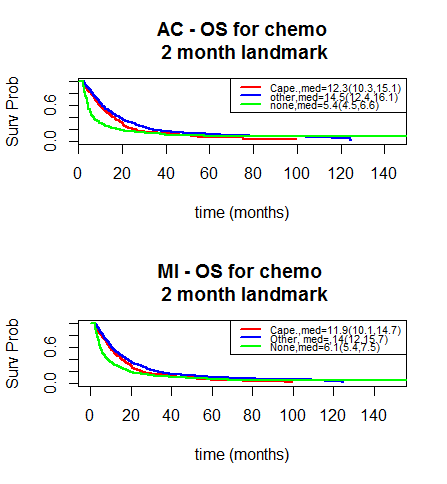
\includegraphics[width=0.8\textwidth]{chemo_km.png}
  \caption{Landmarked Kaplan-Meier curves for chemotherapeutic drugs, AC and MI data}
\label{fig:chemo_km}
\end{figure}


For the HER2 targeted drugs the available case analysis shows that Lapatinib and Trastuzumab are quite close to each other, while having no HER2 directed treatment being much lower. The MI analysis says about the same, but once again gives lower values for the median survival time, as can be seen in figure \ref{fig:her2_km}.

\begin{figure}[h!]
  \centering
    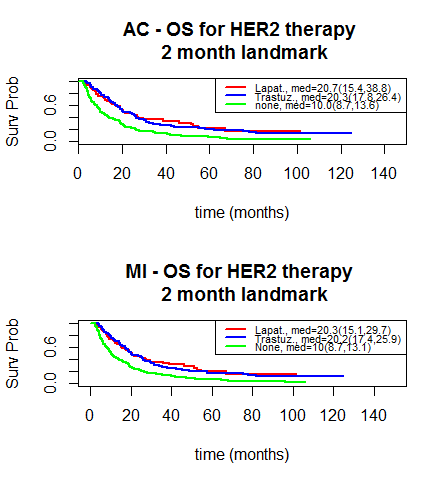
\includegraphics[width=0.8\textwidth]{her2_km.png}
  \caption{Landmarked Kaplan-Meier curves for HER2 drugs, AC and MI data}
\label{fig:her2_km}
\end{figure}

Both Kaplan-Meier curves for both questions seem to show the same thing. As compared to the available case analysis, the estimates of survival are a little pessimistic for the treatments, and a little more optimistic for the no treatment group. This is likely due to the fact that a larger proportion of the missing treatments were assigned to no treatment (which echoes the data), causing their survival to go up. 

Now that we have a visual of the curves, we would like to see if there is actually a difference between them. Although visually, we can see that in both cases, no treatment seems to be much worse for survival than treatment, we need to formalize it. To do so, the log rank test needs to be run on them. We can also get an approximation for the log rank test on the MI data via the Wald test on the pooled Cox model fit only on the treatment. Recall that we are not able to get the exact log rank test because in doing so, we would need to compute either the likelihood ratio test or score test, both of which would include calculating the risk set, which is not possible in the MI setting. It has been suggested to pool the chi square statistics via methods presented in Marshall et al 2009, but even they say that this method is poor \cite{Marshall2009}. So, our only real option is to use the Wald test (which is very easy to compute), and use that value as a proxy for the log rank test (they are asymptotically equivalent).  

The results for the overall test and for each comparison can be seen in table \ref{table:chemo_lr} and  \ref{table:her2_lr}. The AC and MI results are quite similar. For Capecitabine vs other chemo drugs, we see a relatively high p value. Depending on the acceptable rate of significance, different conclusions might be drawn between the two analyses.  In this study, the level is $\alpha=.05$, so changing conclusions is not an issue, however, since we are doing multiple comparisons, it may be prudent to use a Bonferroni correction for multiple testing. For the HER2 directed drugs, there certainly seems to be a difference between the treatments and not having any, but there is no evidence that either of the treatments is better than the other.


\begin{table}[!ht]
\centering
\begin{tabular}{|l|c|c|}
\hline
                & \multicolumn{2}{c|}{Chemo}                         \\ \hline
                & \multicolumn{1}{l|}{AC} & \multicolumn{1}{l|}{MI} \\ \hline
cape/other/none & \textless.0001          & \textless.0001          \\ \hline
cape/other      & 0.0321                  & 0.033                   \\ \hline
cape/none       & 0.00039                 & .0016                   \\ \hline
other/none      & \textless.0001          & \textless.0001          \\ \hline
\end{tabular}
\caption{Chemo log rank tests}
\label{table:chemo_lr}
\end{table}

\begin{table}[!ht]
\centering
\begin{tabular}{|l|c|c|}
\hline
                   & \multicolumn{2}{c|}{HER2}                         \\ \hline
                   & \multicolumn{1}{l|}{AC} & \multicolumn{1}{l|}{MI} \\ \hline
Lapat/Traztuz/none & \textless.0001          & \textless.0001          \\ \hline
Lapat/Trastuz      & .87                     & .81                     \\ \hline
Lapta/none         & .00017                  & .00018                  \\ \hline
Trastuz/none       & \textless.0001          & \textless.0001          \\ \hline
\end{tabular}
\caption{HER2 log rank tests}
\label{table:her2_lr}
\end{table}

Now that we have estimate of the survival curve, we may set up a model to observe how changes in some baseline covariates change the hazard. We will do this with the Cox Proportional Hazards model. Once we have a baseline model fit and the assumptions met, we can add our treatment variable to see how this affects the hazard.  We first need to fit a reasonable model on the available cases. Speaking with the clinicians, they determined that the covariates listed in table \ref{table:importantvars} were clinically relevant for the baseline model. 

We need to make sure that the proportional hazards assumption is met in the available case model to determine if the use of the Cox model is justified. To check, we visually inspect the spline fit to the Schoenfeld residuals over time. The available cases can be seen in figure \ref{fig:ac_schoenfeld}. In the available cases, the assumption of proportional hazards over time seems reasonable, as it a straight line could reasonably be fit between the 95\% confidence bands. A chi square test of correlation also confirms this. 

\begin{figure}[h!]
  \centering
    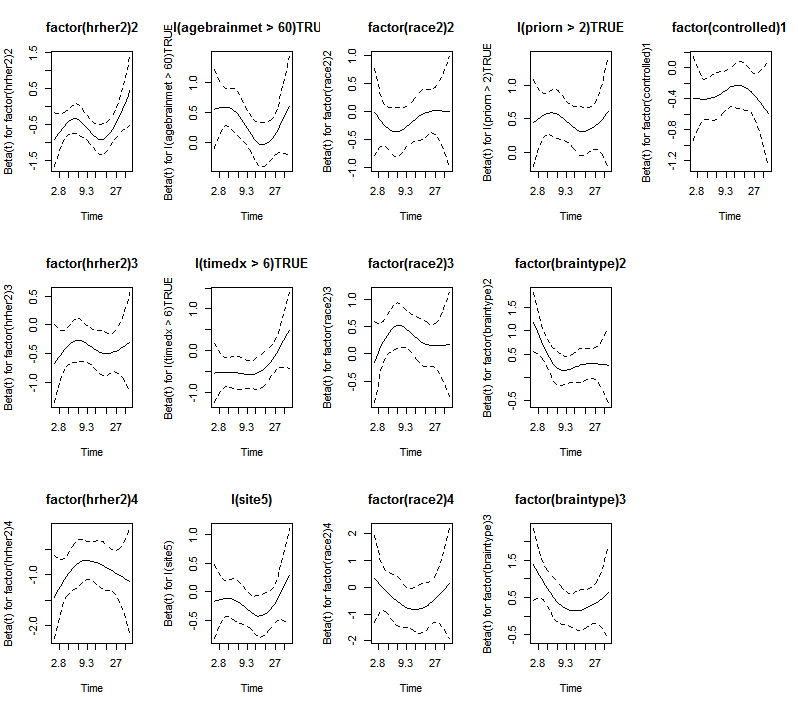
\includegraphics[width=0.8\textwidth]{ac_schoenfeld.png}
  \caption{AC Schoenfeld residuals over time}
\label{fig:ac_schoenfeld}
\end{figure}
Now, to check if we have proportional hazards in the MI data, there are two options. The first is to fit a Cox model on the stacked data, but this will not give us accurate confidence bands. A better option is to collect all of the spline fits, and then superimpose them onto one plot, and assess the shape. This is what is done for the MI data, as can be seen in figure \ref{fig:mi_schoenfeld}. The shapes are very similar to the available cases, so it is reasonable to assume that the proportional hazards assumption holds on the MI data.
\begin{figure}[h!]
  \centering
    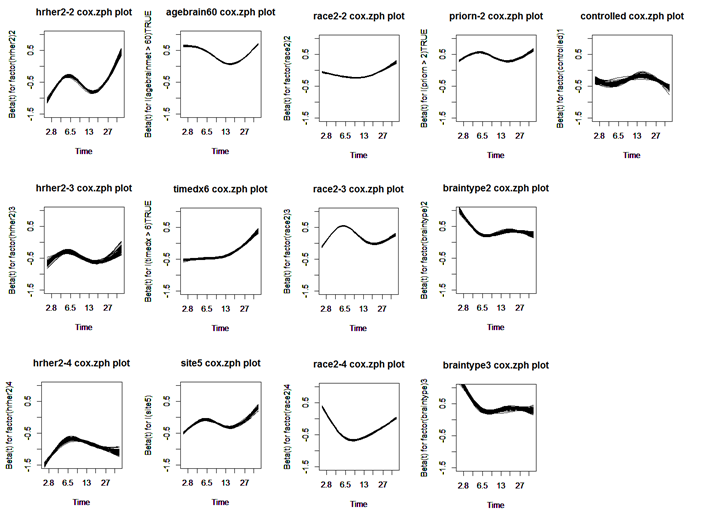
\includegraphics[width=0.8\textwidth]{mi_schoenfeld.png}
  \caption{MI  Schoenfeld residuals over time}
\label{fig:mi_schoenfeld}
\end{figure}


Now that the assumptions are met, we can run the Cox model to obtain the hazard ratios. A table of the AC and MI analyses can be seen in table \ref{fig:acmicox}.




\begin{table}[]
\centering
\begin{tabular}{|c|c|c|c|c|c|c|c|c|}
\hline
                                                       &                                  &      & \begin{tabular}[c]{@{}c@{}}AC \\ n= 845\end{tabular} &                 &  &      & MI                                                 &                                                            \\ \hline
Variable                                               & Contrast                         & HR   & \begin{tabular}[c]{@{}c@{}}95\% \\ CI\end{tabular}   & pvalue          &  & HR   & \begin{tabular}[c]{@{}c@{}}95\% \\ CI\end{tabular} & \begin{tabular}[c]{@{}c@{}}pvalue\\  (t test)\end{tabular} \\ \hline
HR/HER2                                                & -/+ vs. -/-                      & 0.57 & (0.46,0.71)                                          & \textless0.0001 &  & 0.59 & (0.48,0.72)                                        & \textless0.0001                                            \\ \hline
                                                       & +/- vs. -/-                      & 0.66 & (0.54,0.81)                                          & \textless0.0001 &  & 0.63 & (0.52,0.76)                                        & \textless0.0001                                            \\ \hline
                                                       & +/+ vs. -/-                      & 0.4  & (0.31,0.50)                                          & \textless0.0001 &  & 0.4  & (0.32,0.50)                                        & \textless0.0001                                            \\ \hline
Age                                                    & \textgreater 60 vs. \textless 60 & 1.37 & (1.13,1.65)                                          & 0.0011          &  & 1.45 & (1.22,1.72)                                        & \textless0.0001                                            \\ \hline
Dx to BM                                               & \textgreater 6 vs. \textless 6   & 0.66 & (0.54,0.82)                                          & 0.00013         &  & 0.71 & (0.59,0.86)                                        & 0.0002                                                     \\ \hline
First DM                                               & Brain vs. Oth                    & 0.8  & (0.66,0.97)                                          & 0.026           &  & 0.83 & (0.70,0.99)                                        & 0.02                                                       \\ \hline
Race                                                   & Hisp. Vs. White                  & 0.85 & (0.68,1.07)                                          & 0.17            &  & 0.88 & (0.71,1.08)                                        & 0.11                                                       \\ \hline
                                                       & Black vs. White                  & 1.31 & (1.06,1.63)                                          & 0.014           &  & 1.25 & (1.02,1.52)                                        & 0.015                                                      \\ \hline
                                                       & Other vs. White                  & 0.65 & (0.40,1.04)                                          & 0.075           &  & 0.7  & (0.45,1.07)                                        & 0.05                                                       \\ \hline
\begin{tabular}[c]{@{}c@{}}\# prior \\ Rx\end{tabular} & \textgreater2 vs. 0-2            & 1.58 & (1.31,1.91)                                          & \textless0.0001 &  & 1.53 & (1.29,1.82)                                        & \textless0.0001                                            \\ \hline
BM type                                                & Mult. Vs. Single                 & 1.45 & (1.20,1.76)                                          & \textless0.0001 &  & 1.48 & (1.24,1.76)                                        & \textless0.0001                                            \\ \hline
                                                       & LMD vs. Single                   & 1.6  & (1.21,2.13)                                          & 0.001           &  & 1.58 & (1.25,2.00)                                        & \textless0.0001                                            \\ \hline
Sys. Cont.                                             & Yes vs. No                       & 0.71 & (0.61,0.83)                                          & \textless0.0001 &  & 0.73 & (0.63,0.85)                                        & \textless0.0001                                            \\ \hline
\end{tabular}
\caption{AC and MI baseline Cox model}
\label{fig:acmicox}
\end{table}

We may then add in our treatment variable to see how it affects the hazard, and see how it changes other factors. Adding chemotherapy can be seen in \ref{fig:acmichemo}, and for the HER2 positive patients, the HER2 directed drugs can be seen in \ref{fig:acmiher2}. As it has been posited before, the use of chemo and HER2 drugs seem to greatly reduce the hazard ratio of death from cancer. The effect of other covariates in the presence of these drugs seems to change though.
\begin{table}[]
\centering
\begin{tabular}{|c|c|c|c|c|c|c|c|c|}
\hline
            &                                  &      & \begin{tabular}[c]{@{}c@{}}AC\\ n=745\end{tabular} &                 &  &      & MI                                                 &                                                             \\ \hline
Variable    & Contrast                         & HR   & \begin{tabular}[c]{@{}c@{}}95\% \\ CI\end{tabular} & p-value         &  & HR   & \begin{tabular}[c]{@{}c@{}}95\% \\ CI\end{tabular} & \begin{tabular}[c]{@{}c@{}}p-value \\ (t test)\end{tabular} \\ \hline
HR/HER2     & -/+ vs. -/-                      & 0.62 & (0.49,0.79)                                        & \textless .0001 &  & 0.63 & (0.51,0.77)                                        & \textless .0001                                             \\ \hline
            & +/- vs. -/-                      & 0.65 & (0.53,0.81)                                        & 0.00011         &  & 0.64 & (0.53,0.78)                                        & \textless .0001                                             \\ \hline
            & +/+ vs. -/-                      & 0.41 & (0.31,0.53)                                        & \textless .0001 &  & 0.42 & (0.34,0.53)                                        & \textless .0001                                             \\ \hline
Age         & \textgreater 60 vs. \textless 60 & 1.34 & (1.10,1.64)                                        & 0.0041          &  & 1.44 & (1.21,1.72)                                        & \textless .0001                                             \\ \hline
Dx to BM    & \textgreater 6 vs. \textless 6   & 0.72 & (0.58,0.90)                                        & 0.0032          &  & 0.71 & (0.58,0.86)                                        & 0.00039                                                     \\ \hline
First DM    & Brain vs. Oth                    & 0.77 & (0.63,0.95)                                        & 0.014           &  & 0.81 & (0.68,0.96)                                        & 0.016                                                       \\ \hline
Race        & Hisp. Vs. White                  & 0.77 & (0.61,0.98)                                        & 0.034           &  & 0.86 & (0.69,1.06)                                        & 0.15                                                        \\ \hline
            & Black vs. White                  & 1.29 & (1.02,1.63)                                        & 0.032           &  & 1.23 & (1.01,1.51)                                        & 0.043                                                       \\ \hline
            & Other vs. White                  & 0.76 & (0.47,1.25)                                        & 0.28            &  & 0.7  & (0.45,1.08)                                        & 0.11                                                        \\ \hline
\# prior Rx & \textgreater2 vs. 0-2            & 1.61 & (1.32,1.98)                                        & \textless .0001 &  & 1.53 & (1.28,1.82)                                        & \textless .0001                                             \\ \hline
BM type     & Mult. Vs. Single                 & 1.46 & (1.20,1.78)                                        & 0.00017         &  & 1.51 & (1.27,1.81)                                        & \textless .0001                                             \\ \hline
            & LMD vs. Single                   & 1.45 & (1.04,2.03)                                        & 0.029           &  & 1.41 & (1.11,1.80)                                        & 0.0049                                                      \\ \hline
Sys. Cont.  & Yes vs. No                       & 0.57 & (0.48,0.68)                                        & \textless .0001 &  & 0.69 & (0.59,0.80)                                        & \textless .0001                                             \\ \hline
Chemo       & Cape. vs. none            & 0.69 & (0.53,0.89)                                        & 0.0046          &  & 0.75 & (0.60,0.95)                                        & 0.018                                                       \\ \hline
            & other vs. none                   & 0.52 & (0.42,0.65)                                        & \textless .0001 &  & 0.58 & (0.47,0.71)                                        & \textless .0001                                             \\ \hline
\end{tabular}
\caption{AC and MI Cox model with chemo treatment}
\label{fig:acmichemo}
\end{table}

\begin{table}[!ht]
\centering
\begin{tabular}{|c|c|c|c|c|c|c|c|c|}
\hline
             &                                                             &      & \begin{tabular}[c]{@{}c@{}}AC\\ n=292\end{tabular} &                &  &      & MI          &                                                             \\ \hline
Variable     & Contrast                                                    & HR   & 95\% CI                                            & p-value        &  & HR   & 95\% CI     & \begin{tabular}[c]{@{}c@{}}p-value\\  (t test)\end{tabular} \\ \hline
HR/HER2      & +/+ vs. -/+                                                 & 0.65 & (0.49,0.87)                                        & 0.0036         &  & 0.66 & (0.51,0.85) & 0.0015                                                      \\ \hline
Age          & \textgreater 60 vs. \textless 60                            & 1.38 & (0.95,2.01)                                        & 0.092          &  & 1.58 & (1.15,2.18) & 0.0054                                                      \\ \hline
Dx to BM     & \textgreater 6 vs. \textless 6                              & 0.64 & (0.43,0.97)                                        & 0.033          &  & 0.69 & (0.49,0.99) & 0.041                                                       \\ \hline
First DM     & Brain vs. Oth                                               & 0.84 & (0.58,1.20)                                        & 0.34           &  & 0.86 & (0.62,1.17) & 0.34                                                        \\ \hline
Race         & Hisp. Vs. White                                             & 0.69 & (0.46,1.02)                                        & 0.064          &  & 0.76 & (0.53,1.09) & 0.14                                                        \\ \hline
             & Black vs. White                                             & 1.41 & (0.94,2.11)                                        & 0.1            &  & 1.43 & (1.00,2.04) & 0.047                                                       \\ \hline
             & Other vs. White                                             & 0.7  & (0.32,1.53)                                        & 0.38           &  & 0.83 & (0.46,1.52) & 0.55                                                        \\ \hline
\# prior Rx  & \textgreater2 vs. 0-2                                       & 1.88 & (1.34,2.63)                                        & 0.00028        &  & 1.71 & (1.28,2.28) & 0.00028                                                     \\ \hline
BM type      & Mult. Vs. Single                                            & 1.3  & (0.92,1.86)                                        & 0.14           &  & 1.25 & (0.91,1.70) & 0.16                                                        \\ \hline
             & LMD vs. Single                                              & 2.15 & (1.20,3.88)                                        & 0.011          &  & 1.77 & (1.10,2.83) & 0.018                                                       \\ \hline
Sys. Cont.   & Yes vs. No                                                  & 0.73 & (0.55,0.97)                                        & 0.029          &  & 0.78 & (0.60,1.01) & 0.063                                                       \\ \hline
HER2 therapy & \begin{tabular}[c]{@{}c@{}}Lapat vs. \\ none\end{tabular}   & 0.47 & (0.32,0.69)                                        & 0.00015        &  & 0.52 & (0.37,0.75) & 0.00036                                                     \\ \hline
             & \begin{tabular}[c]{@{}c@{}}Trastuz vs. \\ none\end{tabular} & 0.45 & (0.33,0.61)                                        & \textless.0001 &  & 0.51 & (0.38,0.68) & \textless.0001                                              \\ \hline
\end{tabular}
\caption{AC and MI Cox model with HER2 directed treatment, on HER2+ subjects}
\label{fig:acmiher2}
\end{table}
In both analyses, going from available case to MI interpretation, we see that the MI analyses are a little more pessimistic about the hazard ratio. However, the trend in reduction of hazard still holds. Other chemotherapeutics seem to reduce the hazard more than Capecitabine, and Trastuzumab seems to decrease the hazard more than Lapatinib in HER2+ subjects. 

%start here
\section{Causal Analysis}

Lastly, we will want to draw causal inference, and see what the average treatment effect of each drug is.  We will do so by assessing the reduction in hazard via the Cox model. In the previous section, we fit a cox model, but were unable to draw causal conclusions from it since the data was not obtained via an RCT. In this section, we aim to remove the factors confounding treatment and outcome so that we may treat it like an RCT. 

%use ATE and marginal effect interchangeably?	
In order to observe the results from a causal lens, we need to determine what type of treatment effect to look for. It should be noted that some authors use the term marginal to describe population level average effect, and conditional to describe the individual level average effect\cite{Austin2013}. The goal of this study is to make inference about the population, not the individual, so the individual treatment effect is inappropriate. There are two options to choose from in what type of inference to do. There is the ATE (average treatment effect), and the ATT (average treatment effect on the treated). Since we have three comparisons for each group, and there is no clear cut accepted treatment for each, the ATT is not as useful as the ATE, thus we will chose to observe the ATE. 

The idea for this part of the analysis is to use propensity score weighting to create a balanced sample where the baseline covariates are not confounded with treatment assignment, and to be able to treat it as if it was an RCT. Traditional methods to obtain the propensity score (like logistic regression) cannot be optimized for balance. However, machine learning algorithms can be. The method chosen to fit the propensity scores is generalized boosting. In this ensemble method, ``The model consists of many simple regression trees iteratively combined to create an overall piecewise constant function. The iterative fitting algorithm begins with a single simple regression tree, and at each new iteration, another tree is added. The new tree is chosen to provide the best fit to the residuals of the model from the previous iteration'' \cite{McCaffrey2013}. Once a sufficient number of iterations are run, the weights at each iteration are taken and applied to the data, and the balance of the covariates (according to standardized bias or KS statistic) is measured. The iteration that minimizes the bias while not overfitting the data is the model where our final propensity scores are taken from. Standardized bias is more of a measure of central tendency of the groups, whereas the KS statistic is more about the distribution as the whole. Because of this, we will want to optimize on the KS statistic, although both measures should appear balanced after weighting.

In traditional propensity score analysis, there is only one treatment and control, however in our situation, there are actually three groups in each analysis. So we can no longer use methods tailored to two classes. We could fit a multinomial model (that gives probability for three treatment classifications), but the theory behind this is not as strong and easy to understand as with the binary case.  However, if we make treatment status an indicator (for example 1 if treatment is Capecitabine, and 0 if it is other or none), then we may treat it as if it were binary. Because we have three groups though, we will need to check the balance between all groups (i.e 1 vs 2, 1 vs 3, 2 vs 3) to ensure balance is achieved. Since we are summing three probabilities that are not from the same model, we cannot be guaranteed that the probabilities will sum to unity. This is not an issue though, because our primary interest lies in making sure the groups are balanced, not in the sums of the probabilities \cite{McCaffrey2013}. 

We now have the propensity score model selected, but what pretreatment covariates should we control for. In speaking with Dr. Hess, we determined that there are many pretreatment differences in the population that should be controlled for. So even though we wanted to keep the model parsimonious, we were not able to. The covariates we deemed to be important to balance before treatment include: breast cancer stage, race, type of breast cancer, breast cancer surgery site, first metastatic site, number of prior treatments, ECOG score, localized brain mets treatment, type of brain met, age at brain mets, and control of brain mets at diagnosis.

Once the propensity scores have been computed, we need to check that they are in fact valid. McCaffrey et Al. describe two conditions that need to be checked, and graphical checks to do so. The first check is the check of no unmeasured confounders. This is impossible to check, but should be reasonable if we include any and all factors we believe to be confounding. The next condition is to ensure that all of the propensity scores are between 0 and 1. If any propensity score is 0 or 1, then there is no chance that the subject looks like that of another group. If this is the case, then the results will be poor, because the counterfactual framework and propensity score analysis was not meant to handle cases like this \cite{McCaffrey2013}.  All 50 plots for the distribution of the propensity scores cannot be shown in this paper, but I show two. In these plots, figure \ref{fig:pshisto}, we see that the propensity scores are never exactly 0 or 1, and as well, the groups are differentiated, yet still have common support.
\begin{figure}[h!]
\centering
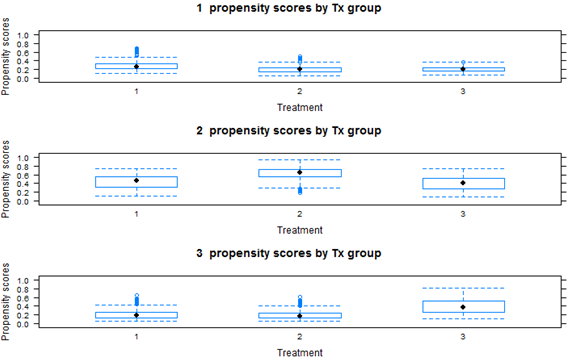
\includegraphics[width=.5\textwidth]{ps_histo1}%
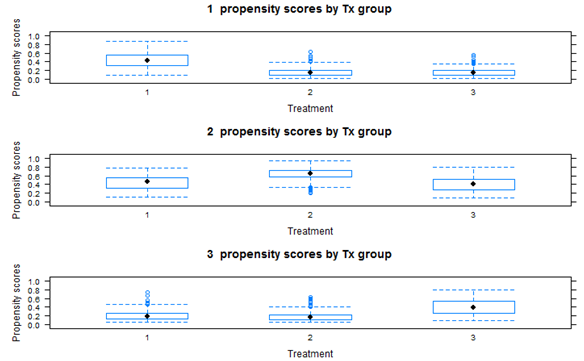
\includegraphics[width=.5\textwidth]{ps_histo2}
  \caption{Selected Propensity Score Histogram Checks}
\label{fig:pshisto}
\end{figure}
To check for balance, we can check how the standardized bias and KS statistic change. Two are selected, as can be seen in figure \ref{fig:psbal}. This plot shows that after weighting, the standardized bias decreases for nearly every variable to an acceptable level (below about .25 is considered balanced in the literature). As well, it shows tthat the KS p-values are increasing, indicating that there is no difference between the distributions of the pretreatment covariates after weighting.


\begin{figure}[h!]
\centering
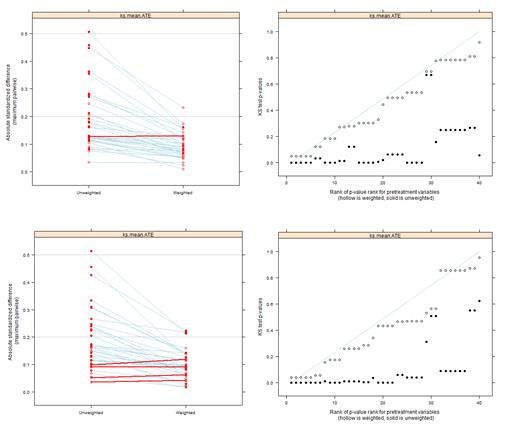
\includegraphics[width=.5\textwidth]{ps_bal_diag}
  \caption{Selected Propensity Score Balance Checks}
\label{fig:psbal}
\medskip
\small
This figure shows how the balance is achieved for two MI datasets. The left hand side denotes the maximum standardized bias for the pretreatment covariates in all groups. The right hand side shows the minimal p-value for the KS test among all groups.
\end{figure}


Once propensity score validity is checked, the weights are put into the Cox model. We cannot be sure that our propensity scores are the truth (this is a known drawback of propensity score analysis), but we can be more confident that it is right by also including the pretreatment covariates as adjustments to the cox model (along with weighting). This is known as being doubly robust estimator \cite{Lunceford2004}.

This is what will happen for one dataset, but since we are in the MI setting, we have 50. The within method discussed before will be our combination plan. This method is chosen since our treatment variable is itself imputed, so this method makes more sense. The idea is to calculate the weighted cox model for each dataset, and then pool. In order to do this though, we need to check the <<balance achieved on each dataset>>. However, once the balance is assessed, we may just pool the results via rubin�s rules. 

After verifying and running the propensity score analysis, the <<results may be seen here>>. As we can see, adjusting for the covariates <<does something>>

!!!EVERYTHING BELOW THIS IS OLD AND WILL PROBABLY GO!!
treatment status, with the Q variables to get our propensity score. We can look at the <standardized bias> before and after the weighting to ensure that we have controlled properly, and to see if we may go forward. Assuming that we have removed the confounding factors and now have two groups that we can treat like it was an RCT, we may now run our Cox model again, but weight by the IPTW. Once we have done this, we can <observe the results from the AC analysis>.

Now we need to apply this propensity score weighting to the MI data. We discussed before the within and across method, and remarked that we were confined to use the within method since our treatment variable (lapat/cape) was itself imputed. So the plan will be to fit the Cox models with the inverse propensity score weights discussed in the AC analysis. We need to be sure that the IPTW weighting is still valid in the MI setting though, so we check <standard biased, other things>. Now we may then pool the results via Rubin's rules and analyze is through the Rubin causal model framework. <the results can be seen here>. The results that we can draw from this are X,Y,Z

\begin{comment}
#mdplot
image(is.na(data), main = "Missing Values", xlab = "Subject",
      ylab = "Variable", 
      xaxt = "n", yaxt = "n", bty = "n",col=c("green","red"))
axis(1, seq(0, 1, length.out = nrow(data)), 1:nrow(data), col = "white")
axis(2,tick=FALSE,labels=FALSE)

#traceplots
plot(imp50x40,c("timemet","timedx","ki67"),main="Traceplots, continuous")
plot(imp50x40,c("controlled","anysys","HER2"),main="Traceplots, binary")
#fluxtable
xtable(subset(j,influx>.3&outflux<.5,select=c("pobs","influx","outflux")))

#chemo km
par(mfcol=c(2,1))
#plot it
#available case
plot(survfit(Surv(os,dead)~capeothno,subset=(os>2),data=data),
     mark.time = FALSE,col=c("red","blue","green"),
     main="Available case OS for chemo\n 2 month landmark",
     xlab="time (months)",ylab="Surv Prob",
     xlim=c(0,150),ylim=c(0,1),lwd=2,xaxt='n')
axis(1, at=c(0,20,40,60,80,100,120,140,160))

legend("topright", 
       legend = c("Cape.,med=12.3(10.3,15.1)",
                  "other,med=14.5(12.4,16.1)",
                  "none,med=5.4(4.5,6.6)"),
       col=c("red","blue","green")
       ,lwd=2,cex=.7)

#mi

plot(capeothno_1_mtx[,1],pooled_KM_est1,type="s",col="red",
     main="MI OS for chemo \n 2 month landmark",
     xlab="time (months)",ylab="Surv Prob",
     xlim=c(0,150),ylim=c(0,1),lwd=2,xaxt='n')
axis(1, at=c(0,20,40,60,80,100,120,140,160))
lines(capeothno_1_mtx[,1],pooled_KM_est2, col="blue",type="s",lwd=2)
lines(capeothno_1_mtx[,1],pooled_KM_est3, col="green",type="s",lwd=2)



legend("topright", legend = c(paste0("Cape.,med=",round(median_time1,1),"(",round(lower_time1,1),",",round(upper_time1,1),")"),
                              paste0("Other, med=,",round(median_time2,1),"(",round(lower_time2,1),",",round(upper_time2,1),")"),
                              paste0("None,med=",round(median_time3,1),"(",round(lower_time3,1),",",round(upper_time3,1),")")),
       col=c("red","blue","green"),lwd=2,cex=.7)

#km for her2
par(mfcol=c(2,1))
#plot it

#available case
plot(survfit(Surv(os,dead)~lapatrasno,subset=(os>2&HER2==1),data=data),
     mark.time=FALSE,
     main="AC - OS for HER2 therapy \n 2 month landmark",
     xlab="time (months)",ylab="Surv Prob",
     xlim=c(0,150),ylim=c(0,1),xaxt='n',lwd=2,col=c("red","blue","green"))
axis(1, at=c(0,20,40,60,80,100,120,140,160))


legend("topright", 
       legend = c("Lapat., med=20.7(15.4,38.8)",
                  "Trastuz., med=20.3(17.8,26.4)",
                  "none, med=10.0(8.7,13.6)"),
       col=c("red","blue","green")
       ,lwd=2,cex=.7)


#MI
plot(lapatrasno_1_mtx[,1],pooled_KM_est1,type="s",col="red",
     main="MI - OS for HER2 therapy \n 2 month landmark",
     xlab="time (months)",ylab="Surv Prob",
     xlim=c(0,150),ylim=c(0,1),xaxt='n',lwd=2)
axis(1, at=c(0,20,40,60,80,100,120,140,160))

lines(lapatrasno_1_mtx[,1],pooled_KM_est2, col="blue",type="s",lwd=2)
lines(lapatrasno_1_mtx[,1],pooled_KM_est3, col="green",type="s",lwd=2)



legend("topright", legend = c(paste0("Lapat., med=",round(median_time1,1),"(",round(lower_time1,1),",",round(upper_time1,1),")"),
                              paste0("Trastuz., med=",round(median_time2,1),"(",round(lower_time2,1),",",round(upper_time2,1),")"),
                              paste0("None, med=",round(median_time3,1),"(",round(lower_time3,1),",",round(upper_time3,1),")")),
       col=c("red","blue","green"),lwd=2,cex=.7)

\end{comment}
